\documentclass[../main.tex]{subfiles}
\begin{document}

\section*{第1問}

% Source: handwritten.pdf 第1問．
{\bf [解]}
$f(x)=px+q-\log x$とおく．$p\leqq0$の時，$f$は連続で
\begin{align}
  f(x)\longrightarrow+\infty\quad(x\to+0),\qquad
  f(x)\longrightarrow-\infty\quad(x\to+\infty)
\end{align}
から，$f(x)=0$なる$x$が存在し不適．よって$p>0$としてよい．
\begin{align}f'(x)=p-\dfrac{1}{x}
\end{align}
より下表である．
\begin{align}
  \begin{array}{c|ccccc}
    x&0&&\dfrac{1}{p}&&\\\hline
    f'&&-&0&+&\\\hline
    f&&\searrow&&\nearrow&
  \end{array}
\end{align}
よって，共有点を持たない条件は
\begin{align}
  f(x)>0\ \Longleftrightarrow\ f\left(\dfrac{1}{p}\right)>0
  \ \Longleftrightarrow\ 1+q+\log p>0\qquad(p>0).
\end{align}
\newpage

\section*{第2問}

% Source: handwritten.pdf 第2問．
{\bf [解]}
$n$秒のあいだに，2頂点$A,B$にしかおとずれない確率を$a_n$，
3頂点$A,B,C$にしかおとずれない確率を$b_n$と定める．
$a_n$について，$P$は$A\to B\to A\to B\to\cdots$の移動をくり返すので，
\begin{align}a_n=\left(\dfrac{1}{3}\right)^n.\label{eq:ky2008-2-a}
\end{align}
対称性から$(A,C)$，$(A,D)$にしかおとずれない確率も$a_n$である．
$b_n$について，常に3頂点のうち上記のごとく2頂点のみに移動をつづけ，
かつ一度は$A,B,C$全てにおとずれることから
\begin{align}
  b_n=\left(\dfrac{2}{3}\right)^n-2a_n
  =\left(\dfrac{2}{3}\right)^n-2\left(\dfrac{1}{3}\right)^n.
  \label{eq:ky2008-2-b}
\end{align}
対称性から，$(A,B,D)$，$(A,C,D)$のみにおとずれる確率も$b_n$である．
以上から，求める確率を$c_n$として，排反から
\begin{align}
  c_n=1-3a_n-3b_n
  =1-3\left\{\left(\dfrac{2}{3}\right)^n-\left(\dfrac{1}{3}\right)^n\right\}.
\end{align}
\newpage

\section*{第3問}

% Source: handwritten.pdf 第3問．
{\bf [解]}
4直線$\ell_k$ $(k=1,2,3,4)$とし，$\ell_k$の方向ベクトルを$\vec{\ell}_k$と表す．
又，$O$を始点とした点$X$の位置ベクトルを$\vec{x}$と表す．
$\ell_k$上に点$A_k$ $(A_k\ne O)$をとり，
\begin{align}\vec{a}_k=t_k\vec{\ell}_k\qquad(t_k\ne0)
\end{align}
と表す．この時$t_k$を適当に定めれば，$A_1A_2A_3A_4$が題意をみたすことを示す．
\begin{figure}[H]
  \begin{center}
    \begin{tikzpicture}[scale=1.1]
      \coordinate (O) at (0,0);
      \foreach \p/\a/\b/\k in {A/-.15/2.0/1,B/1.1/1.6/2,C/2.1/1.0/3,D/1.2/.6/4} {
        \coordinate (\p) at (\a,\b);
        \draw (O)--($(O)!1.3!(\p)$) node[above] {$\ell_{\k}$};
        \fill (\p) circle (1pt) node[above left] {$A_{\k}$};
      }
      \draw (A)--(B)--(C)--(D)--cycle;
      \node[below] at (O) {$O$};
      \begin{scope}[xshift=5cm,yshift=.5cm]
        \coordinate (a) at (0,0); \coordinate (b) at (.6,1.2);
        \coordinate (c) at (2,1.2); \coordinate (d) at (1.4,0);
        \draw (a) node[below left] {$A_1$}--(b) node[above left] {$A_2$}--(c) node[above right] {$A_3$}--(d) node[below right] {$A_4$}--cycle;
        \draw[dashed] (a)--(c);
      \end{scope}
    \end{tikzpicture}
  \end{center}
  \caption{4直線上の交点と，作るべき平行四辺形}
\end{figure}
\begin{align}
  \overrightarrow{A_1A_2}=t_2\vec{\ell}_2-t_1\vec{\ell}_1,\quad
  \overrightarrow{A_1A_4}=t_4\vec{\ell}_4-t_1\vec{\ell}_1,\quad
  \overrightarrow{A_1A_3}=t_3\vec{\ell}_3-t_1\vec{\ell}_1.
  \label{eq:ky2008-3-diff}
\end{align}
$A_1,\ldots,A_4$が条件をみたす時，
$\overrightarrow{A_1A_3}=\overrightarrow{A_1A_2}+\overrightarrow{A_1A_4}$から，
\cref{eq:ky2008-3-diff}を代入して
\begin{align}
  t_3\vec{\ell}_3=t_2\vec{\ell}_2+t_4\vec{\ell}_4-t_1\vec{\ell}_1.
  \label{eq:ky2008-3-linear}
\end{align}
ここで，$\vec{\ell}_k$ $(k=1,2,3)$は互いに一次独立だから，$a,b,c$を定数として
\begin{align}
  \vec{\ell}_3=a\vec{\ell}_1+b\vec{\ell}_2+c\vec{\ell}_3
  \label{eq:ky2008-3-source}
\end{align}
とかける．どの3直線も同一平面上にないので$a,b,c\ne0$だから，
\cref{eq:ky2008-3-linear,eq:ky2008-3-source}より，
\begin{align}a=\dfrac{t_2}{t_3},\qquad b=\dfrac{t_4}{t_3},\qquad c=-\dfrac{t_1}{t_3}
\end{align}
となるよう$t_k$を定めれば良い．よって示された．
% 原稿の式（方向ベクトルの添字）と末尾の係数対応に不整合がある．原稿通り転記し，要確認として記録する．
\newpage

\section*{第4問}

% Source: handwritten.pdf 第4問．
{\bf [解]}
$f(x)=x^2-2$，$g(x)=2x^2+ax-1$とおく．$g(0)=-1<0$から，$g$の2次係数が正なので
$g(x)=0$は必ず2異実根を持ち，
\begin{align}x=\dfrac{-a\pm\sqrt{a^2+8}}{4}
\end{align}
である．これを$\alpha,\beta$ $(\alpha<\beta)$とおく．

\subparagraph{(i) $-\dfrac{3\sqrt{2}}{2}<a<\dfrac{3\sqrt{2}}{2}$の時}
$-\sqrt{2}\leqq\alpha<\beta\leqq\sqrt{2}$となるから，
$x\leqq\alpha$，$\beta\leqq x$に分けて考える．
\begin{figure}[H]
  \begin{center}
    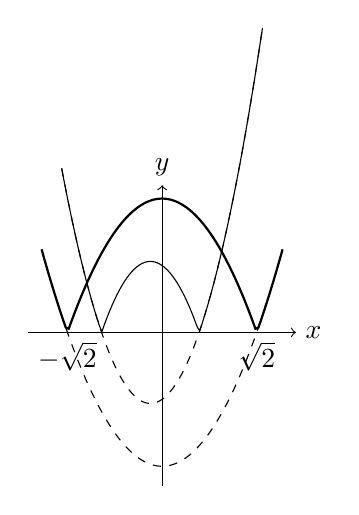
\begin{tikzpicture}[scale=.85]
      \draw[->] (-2,0)--(2,0) node[right] {$x$};\draw[->] (0,-2.3)--(0,2.2) node[above] {$y$};
      \draw[dashed,domain=-1.8:1.8,samples=81] plot(\x,{\x*\x-2});
      \draw[thick,domain=-1.8:1.8,samples=81] plot(\x,{abs(\x*\x-2)});
      \draw[dashed,domain=-1.5:1.5,samples=81] plot(\x,{2*\x*\x+.7*\x-1});
      \draw[domain=-1.5:1.5,samples=81] plot(\x,{abs(2*\x*\x+.7*\x-1)});
      \node[below] at (-1.414,0) {$-\sqrt{2}$};\node[below] at (1.414,0) {$\sqrt{2}$};
    \end{tikzpicture}
  \end{center}
  \caption{$f,g$と絶対値をとったグラフの配置（$|a|<3\sqrt{2}/2$）}
\end{figure}
\subparagraph{(a) $|x|\geqq\sqrt{2}$の時}
\begin{align}
  f(x)=g(x)\ \Longleftrightarrow\ x^2+ax+1=0
  \ \Longleftrightarrow\ x=\dfrac{-a\pm\sqrt{a^2-4}}{2}.
\end{align}
ここで$|a|\leqq\dfrac{3\sqrt{2}}{2}$から
\begin{align}
  \dfrac{-a-\sqrt{a^2-4}}{2}>-\sqrt{2},\qquad
  \dfrac{-a+\sqrt{a^2-4}}{2}<\sqrt{2}
\end{align}
なので，$|x|\geqq\sqrt{2}$の区域に解なし．

\subparagraph{(b) $\alpha<x<\beta$の時}
$|f(x)|=|g(x)|\Longleftrightarrow f(x)=g(x)$であり，(a)からグラフの対応は下図のようになっているので，
\begin{align}
  |a|<2\text{の時 }0\text{つ},\qquad
  |a|=2\text{の時 }1\text{つ},\qquad
  |a|>2\text{の時 }2\text{つ}.
\end{align}
\begin{figure}[H]
  \begin{center}
    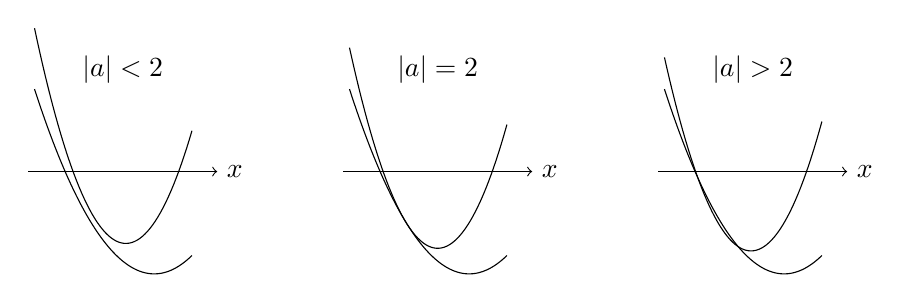
\begin{tikzpicture}[x=.8cm,y=.65cm]
      \foreach \v/\dx/\lab in {1.8/0/{$|a|<2$},2/4/{$|a|=2$},2.1/8/{$|a|>2$}} {
        \begin{scope}[xshift=\dx cm]
          \draw[->] (-2,0)--(1,0) node[right] {$x$};
          \draw[domain=-1.9:.6,samples=61] plot(\x,{\x*\x-2});
          \draw[domain=-1.9:.6,samples=61] plot(\x,{2*\x*\x+\v*\x-1});
          \node at (-.5,2) {\lab};
        \end{scope}
      }
    \end{tikzpicture}
  \end{center}
  \caption{$\alpha<x<\beta$での共有点数の変化}
\end{figure}

\subparagraph{(ii) $\dfrac{3\sqrt{2}}{2}<a$の時}
$\alpha<-\sqrt{2}<\beta<\sqrt{2}$となるから，2次係数に注意してグラフは下図のようになり，4個ある．
\begin{figure}[H]
  \begin{center}
    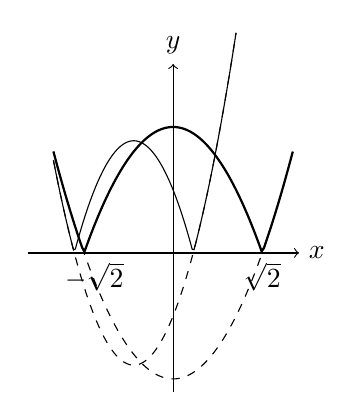
\begin{tikzpicture}[scale=.8]
      \draw[->] (-2.3,0)--(2,0) node[right] {$x$};\draw[->] (0,-2.2)--(0,3) node[above] {$y$};
      \draw[dashed,domain=-1.9:1.9,samples=101] plot(\x,{\x*\x-2});
      \draw[thick,domain=-1.9:1.9,samples=101] plot(\x,{abs(\x*\x-2)});
      \draw[dashed,domain=-1.9:1,samples=101] plot(\x,{2*\x*\x+2.5*\x-1});
      \draw[domain=-1.9:1,samples=101] plot(\x,{abs(2*\x*\x+2.5*\x-1)});
      \node[below] at (-1.25,0) {$-\sqrt{2}$};\node[below] at (1.414,0) {$\sqrt{2}$};
    \end{tikzpicture}
  \end{center}
  \caption{$a>3\sqrt{2}/2$のときの共有点}
\end{figure}

\subparagraph{(iii) $a=\dfrac{3\sqrt{2}}{2}$の時}
$g(x)=2x^2+\dfrac{3\sqrt{2}}{2}x-1$で，グラフは下図で解は3つ．
\begin{figure}[H]
  \begin{center}
    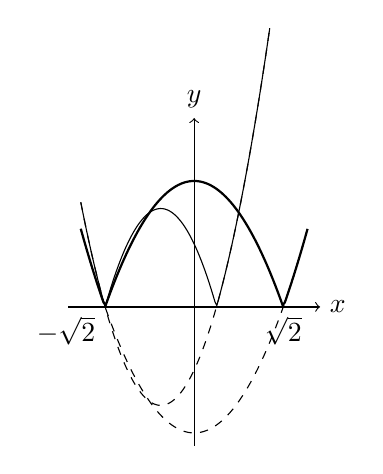
\begin{tikzpicture}[scale=.8]
      \draw[->] (-2,0)--(2,0) node[right] {$x$};\draw[->] (0,-2.2)--(0,3) node[above] {$y$};
      \draw[dashed,domain=-1.8:1.8,samples=101] plot(\x,{\x*\x-2});
      \draw[thick,domain=-1.8:1.8,samples=101] plot(\x,{abs(\x*\x-2)});
      \draw[dashed,domain=-1.8:1.2,samples=101] plot(\x,{2*\x*\x+1.5*sqrt(2)*\x-1});
      \draw[domain=-1.8:1.2,samples=101] plot(\x,{abs(2*\x*\x+1.5*sqrt(2)*\x-1)});
      \node[below left] at (-1.414,0) {$-\sqrt{2}$};\node[below] at (1.414,0) {$\sqrt{2}$};
    \end{tikzpicture}
  \end{center}
  \caption{$a=3\sqrt{2}/2$のときの共有点}
\end{figure}
対称性から$a\leqq-\dfrac{3\sqrt{2}}{2}$についても同様だから，
\begin{align}
  \begin{cases}
    4\text{つ}&a<-\dfrac{3\sqrt{2}}{2},\quad-\dfrac{3\sqrt{2}}{2}<a<-\sqrt{2},\quad
    \sqrt{2}<a<\dfrac{3\sqrt{2}}{2},\quad\dfrac{3\sqrt{2}}{2}<a,\\
    3\text{つ}&a=\pm\dfrac{2\sqrt{2}}{3},\quad\pm2,\\
    2\text{つ}&-\sqrt{2}<a<\sqrt{2}.
  \end{cases}
\end{align}
% 上の最終分類は原稿通り．途中の |a|=2，a=3\sqrt{2}/2 の記述と一致しないので要確認．

\medskip\noindent{\bf [別解]}
\begin{align}
  |f(x)|=|g(x)|&\ \Longleftrightarrow\ 2x^2+ax-1=\pm(x^2-2)\\
  &\ \Longleftrightarrow\ a=\dfrac{-2x^2+1\pm(x^2-2)}{x}\quad(x=0\text{は解でない}),\\
  &\ \Longleftrightarrow\ a=-\left(x+\dfrac{1}{x}\right)\quad\text{又は}\quad
  a=-3x+\dfrac{3}{x}.
\end{align}
グラフから解は分かる．
\begin{figure}[H]
  \begin{center}
    \begin{tikzpicture}[x=.9cm,y=.55cm]
      \draw[->] (-2.6,0)--(2.6,0) node[right] {$x$};\draw[->] (0,-4)--(0,4) node[above] {$y$};
      \begin{scope}
        \clip (-2.5,-3.8) rectangle (2.5,3.8);
        \foreach \lo/\hi in {-2.4/-.28,.28/2.4} {
          \draw[thick,domain=\lo:\hi,samples=81] plot(\x,{-\x-1/\x});
          \draw[domain=\lo:\hi,samples=81] plot(\x,{-3*\x+3/\x});
        }
      \end{scope}
    \end{tikzpicture}
  \end{center}
  \caption{別解における$a=-x-1/x$，$a=-3x+3/x$のグラフ}
\end{figure}
\newpage

\section*{第5問}

% Source: handwritten.pdf 第5問．
{\bf [解]}
$H$の方程式は$z=y-1$である．
$y=2\sin\theta$ $(\dfrac{\pi}{6}\leqq\theta\leqq\dfrac{\pi}{2})$で切断する切り口は下図で，
この面積$S(\theta)$として
\begin{align}S(\theta)=4\cos\theta(2\sin\theta-1).
\end{align}
\begin{figure}[H]
  \begin{center}
    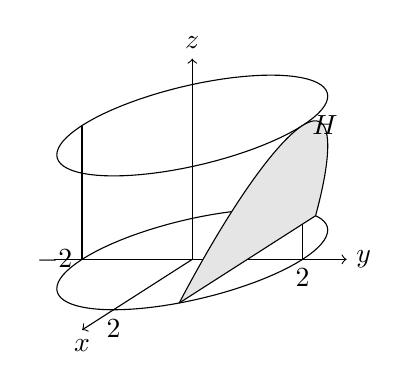
\begin{tikzpicture}[x={(-.5cm,-.32cm)},y={(.7cm,0cm)},z={(0cm,1.7cm)}]
      \draw[->] (0,0,0)--(2.8,0,0) node[below] {$x$};
      \draw[->] (0,-2.5,0)--(0,2.8,0) node[right] {$y$};
      \draw[->] (0,0,0)--(0,0,1.5) node[above] {$z$};
      \draw[domain=0:360,samples=81] plot ({2*cos(\x)},{2*sin(\x)},0);
      \draw[domain=0:360,samples=81] plot ({2*cos(\x)},{2*sin(\x)},1);
      \draw (0,-2,0)--(0,-2,1);\draw (0,2,0)--(0,2,1);
      \fill[gray!20] plot[domain=30:150,samples=61] ({2*cos(\x)},{2*sin(\x)},{2*sin(\x)-1})--cycle;
      \draw[domain=30:150,samples=61] plot ({2*cos(\x)},{2*sin(\x)},{2*sin(\x)-1});
      \draw ({sqrt(3)},1,0)--({-sqrt(3)},1,0);
      \node[right] at (0,2,1) {$H$};\node[below] at (0,2,0) {$2$};
      \node[left] at (0,-2,0) {$-2$};\node[below] at (2,0,0) {$2$};
    \end{tikzpicture}
    \qquad
    \begin{tikzpicture}[scale=.8]
      \fill[pattern=north east lines] (-1.6,0) rectangle (1.6,1.1);
      \draw (-1.6,0) rectangle (1.6,1.1);
      \draw[->] (-2.1,0)--(2.1,0) node[right] {$x$};
      \draw[->] (0,-.4)--(0,1.8) node[above] {$z$};
      \node[below] at (-1.6,0) {$-2\cos\theta$};\node[below] at (1.6,0) {$2\cos\theta$};
      \node[above right] at (0,1.1) {$2\sin\theta-1$};
    \end{tikzpicture}
  \end{center}
  \caption{円柱を平面$H$で分けた部分と$y=2\sin\theta$での切り口}
\end{figure}
だから，以下$c=\cos\theta$，$s=\sin\theta$として，求める体積$V$は
\begin{align}
  \begin{split}
    V&=\int_1^2S(\theta)\,d(2s)\\
    &=\int_{\pi/6}^{\pi/2}S(\theta)\dfrac{d(2s)}{d\theta}\,d\theta\\
    &=\int_{\pi/6}^{\pi/2}4c(2s-1)\,2c\,d\theta\\
    &=8\int_{\pi/6}^{\pi/2}(2c^2s-c^2)\,d\theta\\
    &=8\left[-\dfrac{2}{3}c^3\right]_{\pi/6}^{\pi/2}
    -8\cdot\dfrac{1}{2}\left[\theta+\dfrac{1}{2}\sin2\theta\right]_{\pi/6}^{\pi/2}\\
    &=\dfrac{16}{3}\left(\dfrac{\sqrt{3}}{2}\right)^3
    -4\left(\dfrac{\pi}{3}-\dfrac{1}{2}\cdot\dfrac{\sqrt{3}}{2}\right)\\
    &=3\sqrt{3}-\dfrac{4}{3}\pi.
  \end{split}
\end{align}
\newpage

\section*{第6問}

% Source: handwritten.pdf 第6問．
{\bf [解]}
地球の半径を1として良い．経路$R_1$は，半径$\cos\dfrac{\pi}{3}=\dfrac{1}{2}$の円周のうち
中心角$\dfrac{\pi}{3}$の扇形の弧長で，
\begin{align}R_1=\theta r=\dfrac{1}{2}\cdot\dfrac{1}{3}\pi=\dfrac{1}{6}\pi.\label{eq:ky2008-6-r1}
\end{align}
\begin{figure}[H]
  \begin{center}
    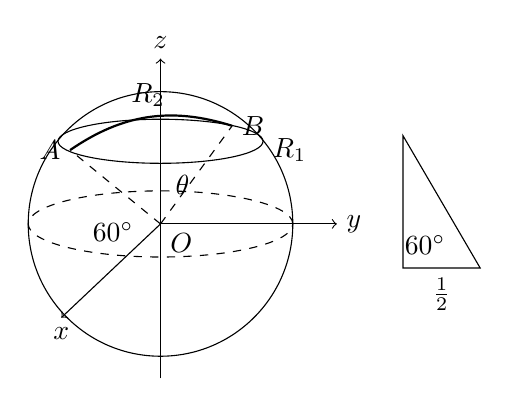
\begin{tikzpicture}[scale=1.4]
      \draw (0,0) circle (1.2);
      \draw[dashed] (0,0) ellipse (1.2 and .3);
      \draw (0,.75) ellipse (.93 and .2);
      \draw[->] (0,-1.4)--(0,1.5) node[above] {$z$};
      \draw[->] (0,0)--(1.6,0) node[right] {$y$};
      \draw[->] (0,0)--(-.9,-.85) node[below] {$x$};
      \coordinate (A) at (-.82,.67);\coordinate (B) at (.65,.89);
      \draw[dashed] (0,0) node[below right] {$O$}--(A) node[left] {$A$};
      \draw[dashed] (0,0)--(B) node[right] {$B$};
      \draw[thick] (A) to[bend left=26] node[above] {$R_2$} (B);
      \node[right] at (.93,.67) {$R_1$};\node at (.2,.35) {$\theta$};
      \node at (-.43,-.07) {$60^\circ$};
      \begin{scope}[xshift=2.2cm,yshift=-.4cm]
        \draw (0,0)--(.7,0) node[midway,below] {$\frac{1}{2}$}--(0,1.2)--cycle;
        \node at (.2,.21) {$60^\circ$};
      \end{scope}
    \end{tikzpicture}
  \end{center}
  \caption{同一緯度の経路$R_1$と大円上の経路$R_2$の模式図}
\end{figure}
一方，$R_2$について，地球の中心を$O$として右のような座標をとれば
\begin{align}
  \overrightarrow{OA}=\dfrac{1}{2}
  \begin{pmatrix}1\\0\\\sqrt{3}
  \end{pmatrix},\qquad
  \overrightarrow{OB}=
  \begin{pmatrix}\dfrac{1}{4}\\\dfrac{\sqrt{3}}{4}\\\dfrac{\sqrt{3}}{2}
  \end{pmatrix}.
\end{align}
だから，$\angle AOB=\theta$として
\begin{align}
  \cos\theta=\dfrac{\overrightarrow{OA}\cdot\overrightarrow{OB}}{|\overrightarrow{OA}|\,|\overrightarrow{OB}|}
  =\dfrac{1}{2}
  \begin{pmatrix}1\\0\\\sqrt{3}
  \end{pmatrix}\cdot
  \dfrac{1}{4}
  \begin{pmatrix}1\\\sqrt{3}\\2\sqrt{3}
  \end{pmatrix}
  =\dfrac{7}{8}=0.875.
\end{align}
三角関数表から，
\begin{align}28.5^\circ<\theta<29.0^\circ.\label{eq:ky2008-6-angle}
\end{align}
\begin{align}R_2=\theta r=\theta.\label{eq:ky2008-6-r2}
\end{align}
したがって，\cref{eq:ky2008-6-r1,eq:ky2008-6-r2}より
\begin{align}\dfrac{R_2}{R_1}<\dfrac{29}{30}=0.96\cdots<0.97,\qquad R_2<0.97R_1
\end{align}
が示された．
\newpage

\end{document}
